%%%%%%%%%%%%%%%%%%%%%% {{{
%%Options for presentations (in-class) and handouts (e.g. print).
\documentclass[pdf,9pt]{beamer}


%%%%%%%%%%%%%%%%%%%%%%
%Change this for different slides so it appears in bar
\usepackage{authoraftertitle}
\date{Chapter 5. Vector Space $\R^n$ \\ \S 5-3. Orthogonality}

%%%%%%%%%%%%%%%%%%%%%%
%% Upload common style file
\usepackage{LyryxLAWASlidesStyle}

\begin{document}

%%%%%%%%%%%%%%%%%%%%%%%
%% Title Page and Copyright Common to All Slides

%Title Page
\input frontmatter/titlepage.tex

%LOTS Page
\input frontmatter/lyryxopentexts.tex

%Copyright Page
\input frontmatter/copyright.tex

%%%%%%%%%%%%%%%%%%%%%%%%% }}}
%-------------- start slide -------------------------------%{{{ 2
\begin{frame}[fragile]
   \tableofcontents
\end{frame}
%-------------- end slide -------------------------------%}}}
\section[\textcolor{yellow}{}]{\textcolor{yellow}{The Dot Product}}
%-------------- start slide -------------------------------%{{{ 1
\frame{
\frametitle{Dot Product}
\pause
\begin{definitions}
  Let $\vec{x}= \left[\begin{array}{c} x_1 \\ x_2 \\ \vdots \\ x_n \end{array}\right]$
  and $\vec{y}= \left[\begin{array}{c} y_1 \\ y_2 \\ \vdots \\ y_n \end{array}\right]$
  be vectors in $\RR^n$.
  \pause
  \begin{enumerate}
    \item The \alert{dot product} of $\vec{x}$ and $\vec{y}$ is
      \[
        \vec{x}\dotprod\vec{y} = x_1y_1 + x_2 y_2 + \cdots x_n y_n = \vec{x}^T\vec{y}.
      \]
    \pause
    \item The \alert{length} or \alert{norm} of $\vec{x}$, denoted
      $||\vec{x}||$ is
      \[
        ||\vec{x}|| = \sqrt{x_1^2 + x_2^2 \cdots + x_n^2} = \sqrt{\vec{x}\dotprod\vec{x}} = \sqrt{\vec{x}^T \vec{x}}.
      \]
    \pause
    \item $\vec{x}$ is called a \alert{unit vector} if $||\vec{x}||=1$.
  \end{enumerate}
\end{definitions}
}
%-------------- end slide -------------------------------%}}}
%-------------- start slide -------------------------------%{{{ 2
\frame{
\begin{theorem}[Properties of length and the dot product]
Let $\vec{x},\vec{y},\vec{z}\in\RR^n$, and let $a\in\RR$.
Then
\pause
\begin{enumerate}
  \item $\vec{x}\dotprod\vec{y} =\vec{y}\dotprod\vec{x}$
    \textcolor{blue}{(the dot product is commutative)}
  \pause
  \item $\vec{x}\dotprod(\vec{y}+\vec{z}) =\vec{x}\dotprod\vec{y} +
    \vec{x}\dotprod\vec{z}$
    \textcolor{blue}{(the dot product distributes over addition)}
  \pause
  \item $(a\vec{x})\dotprod\vec{y} =a(\vec{x}\dotprod\vec{y})= \vec{x}\dotprod(a\vec{y})$
  \pause
  \item $||\vec{x}||^2=\vec{x}\dotprod\vec{x}$.
  \pause
  \item $||\vec{x}||\geq 0$ with equality if and only if $\vec{x}=\vec{0}_n$.
  \pause
  \item $||a\vec{x}||=|a|~||\vec{x}||$.
\end{enumerate}
\end{theorem}
}
%-------------- end slide -------------------------------%}}}
%-------------- start slide -------------------------------%{{{ 3
\frame{
\begin{example}
Let $\vec{x},\vec{y}\in\RR^n$.
Then
\begin{eqnarray*}
  ||\vec{x}+\vec{y}||^2 & = & (\vec{x}+\vec{y})\dotprod (\vec{x}+\vec{y})                                                             \\
                          & = & \vec{x}\dotprod \vec{x} + \vec{x}\dotprod\vec{y} + \vec{y}\dotprod \vec{x} + \vec{y}\dotprod\vec{y} \\
                          & = & \vec{x}\dotprod\vec{x} + 2(\vec{x}\dotprod\vec{y}) + \vec{y}\dotprod\vec{y}                           \\
                          & = & ||\vec{x}||^2 + 2(\vec{x}\dotprod\vec{y}) + ||\vec{y}||^2.
\end{eqnarray*}
\end{example}
}
%-------------- end slide -------------------------------%}}}
%-------------- start slide -------------------------------%{{{ 4
\frame{
\begin{problem}
    Let $\{\vec{f}_1, \vec{f}_2, \ldots, \vec{f}_k\}\in\RR^n$ and
    suppose $\RR^n=\Span\{\vec{f}_1, \vec{f}_2, \ldots, \vec{f}_k\}$.
    Furthermore, suppose that there exists a vector $\vec{x}\in\RR^n$
    for which $\vec{x}\dotprod\vec{f}_j=0$ for all $j$, $1\leq j\leq k$.
    Show that $\vec{x}=\vec{0}_n$.
\end{problem}
    \pause
    \vfill
\begin{proofnoend}
    Write $\vec{x}=t_1\vec{f}_1 + t_2\vec{f}_2 +\cdots +t_k\vec{f}_k$
    for some $t_1, t_2, \ldots, t_k\in\RR$
    \textcolor{blue}{(this is possible because $\vec{f}_1, \vec{f}_2, \ldots,
    \vec{f}_k$ span $\RR^n$, is this representation unique?).}
    \pause
    Then
    \begin{eqnarray*}
    ||\vec{x}||^2 & = & \vec{x}\dotprod\vec{x} \\ \pause
		 & = & \vec{x}\dotprod(t_1\vec{f}_1 + t_2\vec{f}_2 +\cdots +t_k\vec{f}_k) \\ \pause
		 & = & \vec{x}\dotprod (t_1\vec{f}_1) +  \vec{x}\dotprod (t_2\vec{f}_2) + \cdots +  \vec{x}\dotprod (t_k\vec{f}_k) \\ \pause
		 & = & t_1(\vec{x}\dotprod\vec{f}_1) + t_2(\vec{x}\dotprod\vec{f}_2) + \cdots + t_k(\vec{x}\dotprod\vec{f}_k) \\ \pause
		 & = & t_1(0) + t_2(0) + \cdots + t_k(0) = 0.
    \end{eqnarray*}
    \pause
    Since $||\vec{x}||^2 =0$, $||\vec{x}|| =0$.
    By the previous theorem,  $||\vec{x}|| =0$ if and only if
    $\vec{x}=\vec{0}_n$.
    Therefore, $\vec{x}=\vec{0}_n$.
    \myQED
\end{proofnoend}
}
%-------------- end slide -------------------------------%}}}
\section[\textcolor{yellow}{}]{\textcolor{yellow}{The Cauchy Inequality}}
%-------------- start slide -------------------------------%{{{ 5
\frame{
\frametitle{Cauchy-Schwartz Inequality}
\pause
\begin{theorem}[Cauchy-Schwartz Inequality]
    If $\vec{x},\vec{y}\in\RR^n$, then $|\vec{x}\dotprod\vec{y}|\leq ||\vec{x}||~||\vec{y}||$
     with equality if and only if $\{\vec{x},\vec{y}\}$ is linearly dependent.
\end{theorem}
\vfill
\begin{minipage}{0.49\textwidth}
\begin{center}
    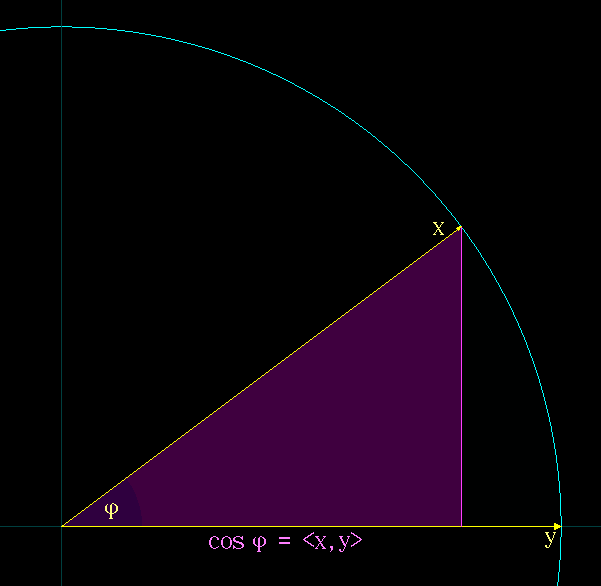
\includegraphics[scale=0.15]{./figures/Cauchy-Schwarz_inequation_in_Euclidean_plane.png}
\end{center}
\end{minipage}
\begin{minipage}{0.49\textwidth}
    \begin{align*}
	\left| \frac{\vec{x}}{||\vec{x}||} \cdot \frac{\vec{y}}{||\vec{y}||} \right| \le 1
    \end{align*}
\end{minipage}
\vfill
\begin{emptytitle}
\begin{align*}
    \text{$\{\vec{x},\vec{y}\}$ is linearly dependent} \quad
    \Leftrightarrow \quad \vec{x} = t \vec{y},\quad \text{for some~} t\in\R.
\end{align*}
\end{emptytitle}
}
%-------------- end slide -------------------------------%}}}
%-------------- start slide -------------------------------%{{{ 6
\begin{frame}[fragile]
\begin{proofnoend}
    Let $\vec{x},\vec{y}\in\RR^n$ and $t\in\RR$.
    Then
    \begin{eqnarray*}
	0\leq ||t\vec{x}+\vec{y}||^2
	& = &  (t\vec{x}+\vec{y})\dotprod (t\vec{x}+\vec{y}) \\
	& = &  t^2\vec{x}\dotprod\vec{x}+ 2t\vec{x}\dotprod\vec{y} +\vec{y}\dotprod\vec{y}\\
	& = &  t^2||\vec{x}||^2+ 2t(\vec{x}\dotprod\vec{y}) +||\vec{y}||^2.
    \end{eqnarray*}
    The quadratic $t^2||\vec{x}||^2+ 2t(\vec{x}\dotprod\vec{y}) +||\vec{y}||^2$
    in $t$ is always nonnegative, so it does not have distinct real roots.
    Thus, if we use the quadratic formula to solve for $t$, the discriminant
    must be non-positive, i.e.,
    \begin{align*}
       \Delta = (2\vec{x}\dotprod\vec{y})^2-4||\vec{x}||^2 ||\vec{y}||^2 \leq 0
    \end{align*}
    Therefore,
    $(2\vec{x}\dotprod\vec{y})^2\leq 4||\vec{x}||^2||\vec{y}||^2$.
    Since both sides of the inequality are nonnegative, we can take
    (positive) square roots of both sides:
    \[ |2\vec{x}\dotprod\vec{y}|\leq 2||\vec{x}||~||\vec{y}||\]
    Therefore,
    $|\vec{x}\dotprod\vec{y}|\leq ||\vec{x}||~||\vec{y}||$.
    What remains is to show that
    $|\vec{x}\dotprod\vec{y}|=||\vec{x}||~||\vec{y}||$
    if and only if $\{\vec{x},\vec{y}\}$ is linearly dependent.
    \myQED
\end{proofnoend}
\end{frame}
%-------------- end slide -------------------------------%}}}
%-------------- start slide -------------------------------%{{{ 7
\frame{
\begin{proofnoend}[continued]
    First suppose that $\{\vec{x},\vec{y}\}$ is dependent.
    Then by symmetry (of $\vec{x}$ and $\vec{y}$),
    $\vec{x}=k\vec{y}$ for some $k\in\RR$.
    Hence
    \[ |\vec{x}\dotprod\vec{y}| = |(k\vec{y})\dotprod\vec{y}|
	=|k|~|\vec{y}\dotprod\vec{y}|
	= |k|~||\vec{y}||^2,\quad\text{and}\quad
	||\vec{x}||~||\vec{y}||= ||k\vec{y}||~||\vec{y}||
    =|k|~||\vec{y}||^2, \]
    so $|\vec{x}\dotprod\vec{y}|=||\vec{x}||~||\vec{y}||$.
    \medskip

    Conversely, suppose $\{\vec{x},\vec{y}\}$ is independent;
    then $t\vec{x}+\vec{y}\neq\vec{0}_n$ for all $t\in\RR$,
    so $||t\vec{x}+\vec{y}||^2>0$ for all $t\in\RR$.
    Thus the quadratic
    \[ t^2||\vec{x}||^2+ 2t(\vec{x}\dotprod\vec{y}) +||\vec{y}||^2 >0\]
    so has no real roots.
    It follows that the the discriminant is
    negative, i.e.,
    % \vspace*{-.15in}

    \[ (2\vec{x}\dotprod\vec{y})^2-4||\vec{x}||^2 ||\vec{y}||^2 < 0.\]
    Therefore,
    $(2\vec{x}\dotprod\vec{y})^2<4||\vec{x}||^2 ||\vec{y}||^2$;
    taking square roots of both sides
    (they are both nonnegative) and dividing by two gives us
    % \vspace*{-.15in}

    \[ |\vec{x}\dotprod\vec{y}|< ||\vec{x}||~||\vec{y}||,\]
    showing that equality is impossible.
    \myQED
\end{proofnoend}
}
%-------------- end slide -------------------------------%}}}
%-------------- start slide -------------------------------%{{{ 8
\frame{
\begin{corollary}[Triangle Inequality I ]
If $\vec{x},\vec{y}\in\RR^n$, then
$||\vec{x}+\vec{y}||\leq ||\vec{x}|| + ||\vec{y}||$.
\end{corollary}
\pause
\begin{proofnoend}
\begin{eqnarray*}
||\vec{x}+\vec{y}||^2 & = & (\vec{x}+\vec{y})\dotprod (\vec{x}+\vec{y}) \\
\pause
& = & \vec{x}\dotprod\vec{x} + 2\vec{x}\dotprod\vec{y} +
\vec{y}\dotprod\vec{y} \\
\pause
& = & ||\vec{x}||^2 + 2\vec{x}\dotprod\vec{y} + ||\vec{y}||^2 \\
\pause
& \leq & ||\vec{x}||^2 + 2||\vec{x}||~||\vec{y}|| + ||\vec{y}||^2
\mbox{ by the Cauchy Inequality} \\
\pause
& = & ( ||\vec{x}|| + ||\vec{y}||)^2.
\end{eqnarray*}
\pause
Since both sides of the inequality are nonnegative, we
take (positive) square roots of both sides:
\[ ||\vec{x}+\vec{y}||\leq ||\vec{x}|| + ||\vec{y}||.\]
\myQED\end{proofnoend}
}
%-------------- end slide -------------------------------%}}}
%-------------- start slide -------------------------------%{{{ 9
\frame{
\begin{definition}
    If $\vec{x},\vec{y}\in\RR^n$, then the \alert{distance} between
    $\vec{x}$ and $\vec{y}$ is defined as
    \[ \alert{d(\vec{x},\vec{y})= ||\vec{x}-\vec{y}||.}\]
\end{definition}
\pause
\begin{theorem}[Properties of the distance function]
    Let $\vec{x},\vec{y},\vec{z}\in\RR^n$.  Then
    \pause
    \begin{enumerate}
	\item $d(\vec{x},\vec{y}) \geq 0$.  \pause
	\item $d(\vec{x},\vec{y}) =0$ if and only if $\vec{x}=\vec{y}$.  \pause
	\item $d(\vec{x},\vec{y}) = d(\vec{y},\vec{x})$.  \pause
	\item $d(\vec{x},\vec{z}) \leq d(\vec{}x,\vec{y}) + d(\vec{y},\vec{z})$ \textcolor{blue}{(Triangle Inequality II)}.
    \end{enumerate}
\end{theorem}
\pause
\begin{proofnoend}[Proof of the Triangle Inequality II]
    \begin{eqnarray*}
	d(\vec{x},\vec{z}) = ||\vec{x}-\vec{z}|| & =    & ||(\vec{x}-\vec{y}) +(\vec{y}-\vec{z})||                                  \\ \pause
						 & \leq & ||\vec{x}-\vec{y}|| +||\vec{y}-\vec{z}|| \mbox{ by Triangle Inequality I} \\ \pause
						 & =    & d(\vec{x},\vec{y}) + d(\vec{y},\vec{z}).
    \end{eqnarray*}
    \myQED
\end{proofnoend}
}
%-------------- end slide -------------------------------%}}}
\section[\textcolor{yellow}{}]{\textcolor{yellow}{Orthogonality}}
%-------------- start slide -------------------------------%{{{ 10
\frame{
\frametitle{Orthogonality}
\pause
\begin{definitions}
  \begin{itemize}
    \item Let $\vec{x},\vec{y}\in\RR^n$.  We say that two vectors $\vec{x}$ and
	$\vec{y}$ are \alert{orthogonal} if $\vec{x}\dotprod\vec{y}=0$.\\[0.5em]
    \pause
    \item More generally, $X=\{\vec{x}_1, \vec{x}_2, \ldots,
      \vec{x}_k\}\subseteq\RR^n$ is an \alert{orthogonal set} if each
      $\vec{x_i}$ is nonzero, and every pair of \textcolor{blue}{distinct}
      vectors of $X$ is orthogonal, i.e., $\vec{x}_i\dotprod \vec{x}_j=0$ for
      all $i\neq j$, $1\leq i,j\leq k$.\\[0.5em]
    \pause
    \item A set $X=\{\vec{x}_1, \vec{x}_2, \ldots,
      \vec{x}_k\}\subseteq\RR^n$ is an \alert{orthonormal} set if $X$ is an
      orthogonal set of \textcolor{blue}{unit vectors}, i.e.,
      $||\vec{x_i}||=1$ for all $i$, $1\leq i\leq k$.
  \end{itemize}
\end{definitions}
}
%-------------- end slide -------------------------------%}}}
%-------------- start slide -------------------------------%{{{ 11
\frame{
\begin{examples}
    \begin{enumerate}
	\item The standard basis $\{\vec{e}_1,\cdots,\vec{e}_n\}$ of $\RR^n$ is an orthonormal set (and hence an orthogonal set).
	\pause
	\bigskip
	\item
	\[\footnotesize \left\{
	    \left[\begin{array}{r} 1 \\ 1 \\ 1 \\ 1 \end{array}\right],
	    \left[\begin{array}{r} 1 \\ 1 \\ -1 \\ -1 \end{array}\right],
	    \left[\begin{array}{r} 1 \\ -1 \\ 1 \\ -1 \end{array}\right]
	\right\}\]
	is an orthogonal (but not orthonormal) subset of $\RR^4$.
	\pause
	\bigskip
	\item If $\{ \vec{x}_1, \vec{x}_2, \ldots, \vec{x}_k\}$
	is an orthogonal subset of $\RR^n$ and $p\neq 0$, then
	$\{ p\vec{x}_1, p\vec{x}_2, \ldots, p\vec{x}_k\}$
	is an orthogonal subset of $\RR^n$.
	\pause
	\bigskip
	\item
	\[ \footnotesize \left\{
	    \frac{1}{2}\left[\begin{array}{r} 1 \\ 1 \\ 1 \\ 1 \end{array}\right],
	    \frac{1}{2}\left[\begin{array}{r} 1 \\ 1 \\ -1 \\ -1 \end{array}\right],
	    \frac{1}{2}\left[\begin{array}{r} 1 \\ -1 \\ 1 \\ -1 \end{array}\right]
	\right\}\]
	is an orthonormal subset of $\RR^4$.
    \end{enumerate}
\end{examples}
}
%-------------- end slide -------------------------------%}}}
%-------------- start slide -------------------------------%{{{ 12
\frame{
\begin{definition}
    \alert{Normalizing an orthogonal set} is the process of
    turning an orthogonal (but not orthonormal) set into
    an orthonormal set.
    If $\{ \vec{x}_1, \vec{x}_2, \ldots, \vec{x}_k\}$
    is an orthogonal subset of $\RR^n$,
    then
    \[ \left\{
	\frac{1}{||\vec{x}_1||}\vec{x}_1,
	\frac{1}{||\vec{x}_2||}\vec{x}_2, \ldots,
	\frac{1}{||\vec{x}_k||}\vec{x}_k \right\}
    \]
    is an orthonormal set.
\end{definition}
}
%-------------- end slide -------------------------------%}}}
%-------------- start slide -------------------------------%{{{ 13
\begin{frame}[fragile]
   \begin{center}
       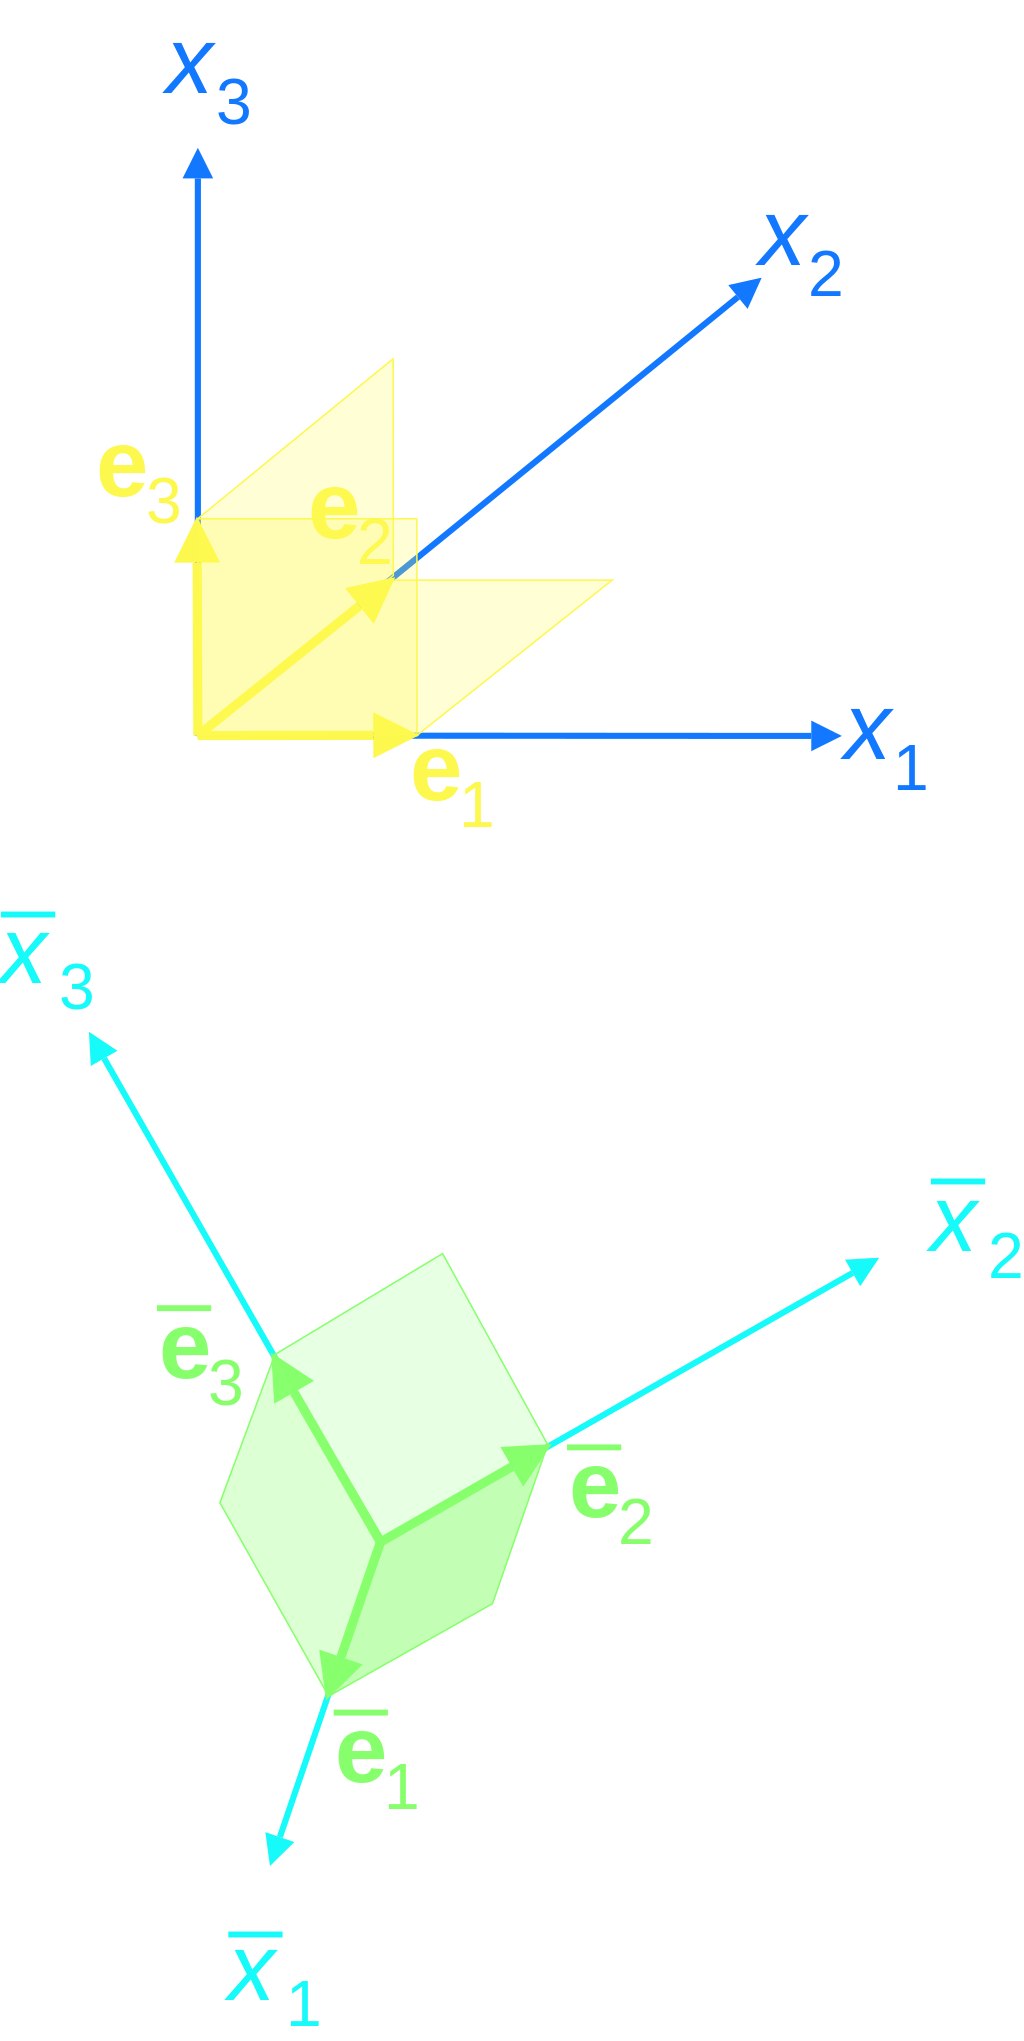
\includegraphics[scale=0.1]{./figures/Rectangular_coordinate_systems_index_lowered.png}
   \end{center}
\end{frame}
%-------------- end slide -------------------------------%}}}
%-------------- start slide -------------------------------%{{{ 14
\begin{frame}[fragile]
\begin{problem}
    Verify that
    \[ \left\{
      \left[\begin{array}{r} 1 \\ -1 \\ 2 \end{array}\right],
      \left[\begin{array}{r} 0 \\ 2 \\ 1  \end{array}\right],
      \left[\begin{array}{r} 5 \\ 1 \\ -2 \end{array}\right]
    \right\} \]
    is an orthogonal set, and normalize this set.
\end{problem}
\end{frame}
%-------------- end slide -------------------------------%}}}
%-------------- start slide -------------------------------%{{{ 15
\frame{
\begin{solution}
  \begin{eqnarray*}
    \left[\begin{array}{r} 1 \\ -1 \\ 2 \end{array}\right]\dotprod
    \left[\begin{array}{r} 0 \\ 2 \\ 1  \end{array}\right]
    & = & 0 - 2 + 2 = 0, \\
    \left[\begin{array}{r} 0 \\ 2 \\ 1  \end{array}\right]\dotprod
    \left[\begin{array}{r} 5 \\ 1 \\ -2 \end{array}\right]
    & = & 0 + 2 - 2 = 0, \\
    \left[\begin{array}{r} 1 \\ -1 \\ 2 \end{array}\right]\dotprod
    \left[\begin{array}{r} 5 \\ 1 \\ -2 \end{array}\right]
    & = & 5 - 1 - 4 = 0 ,
  \end{eqnarray*}
  proving that the set is orthogonal.
  Normalizing gives us the orthonormal set
  \[
  \left\{
    \frac{1}{\sqrt{6}}\left[\begin{array}{r}  1 \\ -1 \\ 2  \end{array}\right],
    \frac{1}{\sqrt{5}}\left[\begin{array}{r}  0 \\ 2  \\ 1  \end{array}\right],
    \frac{1}{\sqrt{30}}\left[\begin{array}{r} 5 \\ 1  \\ -2 \end{array}\right]
  \right\}.
  \]
  \myQED
\end{solution}
}
%-------------- end slide -------------------------------%}}}
%-------------- start slide -------------------------------%{{{ 16
\frame{
\begin{theorem}[Pythagoras' Theorem]
  If $\{ \vec{x}_1, \vec{x}_2, \ldots, \vec{x}_k\}\subseteq\RR^n$
  is orthogonal, then
  \[ || \vec{x}_1 + \vec{x}_2 + \cdots + \vec{x}_k||^2
  = || \vec{x}_1||^2 +|| \vec{x}_2 ||^2 + \cdots + || \vec{x}_k ||^2.\]
\end{theorem}
\pause
\vfill
\begin{proofnoend}
    Start with
    \begin{eqnarray*}
      || \vec{x}_1 + \vec{x}_2 + \cdots + \vec{x}_k||^2
      & = &  (\vec{x}_1 + \vec{x}_2 + \cdots + \vec{x}_k) \dotprod (\vec{x}_1 + \vec{x}_2 + \cdots + \vec{x}_k) \\ \pause
      & = & \phantom{+ }(\textcolor{red}{\vec{x}_1\dotprod\vec{x}_1} + \vec{x}_1\dotprod\vec{x}_2 + \cdots + \vec{x}_1\dotprod\vec{x}_k)    \\
      &   & + (\vec{x}_2\dotprod\vec{x}_1 + \textcolor{red}{\vec{x}_2\dotprod\vec{x}_2} + \cdots + \vec{x}_2\dotprod\vec{x}_k)  \\
      &   & ~~~\vdots\hspace*{1in}\vdots\hspace*{1in}\vdots                                                          \\
      &   & + (\vec{x}_k\dotprod\vec{x}_1 + \vec{x}_k\dotprod\vec{x}_2 + \cdots + \textcolor{red}{\vec{x}_k\dotprod\vec{x}_k})  \\
      & = &  \alert{\vec{x}_1\dotprod\vec{x}_1}+ \alert{\vec{x}_2\dotprod \vec{x}_2} + \cdots +  \alert{\vec{x}_k\dotprod\vec{x}_k}\\ \pause
      & = & || \vec{x}_1||^2 +|| \vec{x}_2 ||^2 + \cdots + || \vec{x}_k ||^2.
    \end{eqnarray*}
  % \vspace*{-.2in}

  \pause
  The second last equality follows from the fact that the set is
  orthogonal, so for all $i$ and $j$, $i\neq j$ and
  $1\leq i, j\leq k$, $\vec{x}_i\dotprod\vec{x}_j=0$.
  Thus, the only nonzero terms are the ones of the form
  $\vec{x}_i\dotprod\vec{x}_i$, $1\leq i\leq k$.
  \myQED
\end{proofnoend}
}
%-------------- end slide -------------------------------%}}}
\section[\textcolor{yellow}{}]{\textcolor{yellow}{Orthogonality and Independence}}
%-------------- start slide -------------------------------%{{{ 17
\frame{
\frametitle{Orthogonality and Independence}
\pause
\begin{theorem}
    If $S= \{ \vec{x}_1, \vec{x}_2, \ldots, \vec{x}_k\}\subseteq\RR^n$
    is an orthogonal set, then $S$ is independent.
\end{theorem}
\pause
\vfill
\begin{proofnoend}
    Form the linear equation: $t_1\vec{x}_1 + t_2\vec{x}_2 + \cdots +
    t_k\vec{x}_k=\vec{0}$. We need to check whether there is only trivial
    solution.
    \pause
    Notice that for all $i$, $1\leq i\leq k$,
    \[ 0 = (t_1\vec{x}_1 + t_2\vec{x}_2 + \cdots + t_k\vec{x}_k)\dotprod
    \vec{x}_i = t_i\vec{x}_i\dotprod\vec{x}_i =t_i||\vec{x}_i||^2, \]
    since $t_j\vec{x}_j\dotprod \vec{x}_i=0$ for all $j$,
    $1\leq j\leq k$ where $j\neq i$.
    \pause
    Since $\vec{x}_i\neq\vec{0}_n$ and $t_i||\vec{x}_i||^2=0$, it follows
    that $t_i=0$ for all $i$, $1\leq i\leq k$.
    Therefore, $S$ is linearly independent.
    \myQED
\end{proofnoend}
}
%-------------- end slide -------------------------------%}}}
%-------------- start slide -------------------------------%{{{ 18
\frame{
\begin{example}
    Given an arbitrary vector
    \[ \vec{x}=\left[\begin{array}{c} a_1 \\ a_2 \\ \vdots \\ a_n
    \end{array}\right] \in \RR^n,\] it is trivial to express
    $\vec{x}$ as a linear combination of the standard basis
    vectors of $\RR^n$,
    $\{ \vec{e}_1, \vec{e}_2, \ldots, \vec{e}_n\}$:
    \[ \vec{x} = a_1\vec{e}_1 + a_2\vec{e}_2 + \cdots + a_n\vec{e}_n.\]
\end{example}
}
%-------------- end slide -------------------------------%}}}
%-------------- start slide -------------------------------%{{{ 19
\begin{frame}[fragile]
\begin{problem}
    Given any orthogonal basis $B$ of $\RR^n$ (so not necessarily
    the standard basis), and an arbitrary vector $\vec{x}\in\RR^n$,
    how do we express $\vec{x}$ as a linear combination of the
    vectors in $B$?
\end{problem}
\vfill
\begin{center}
   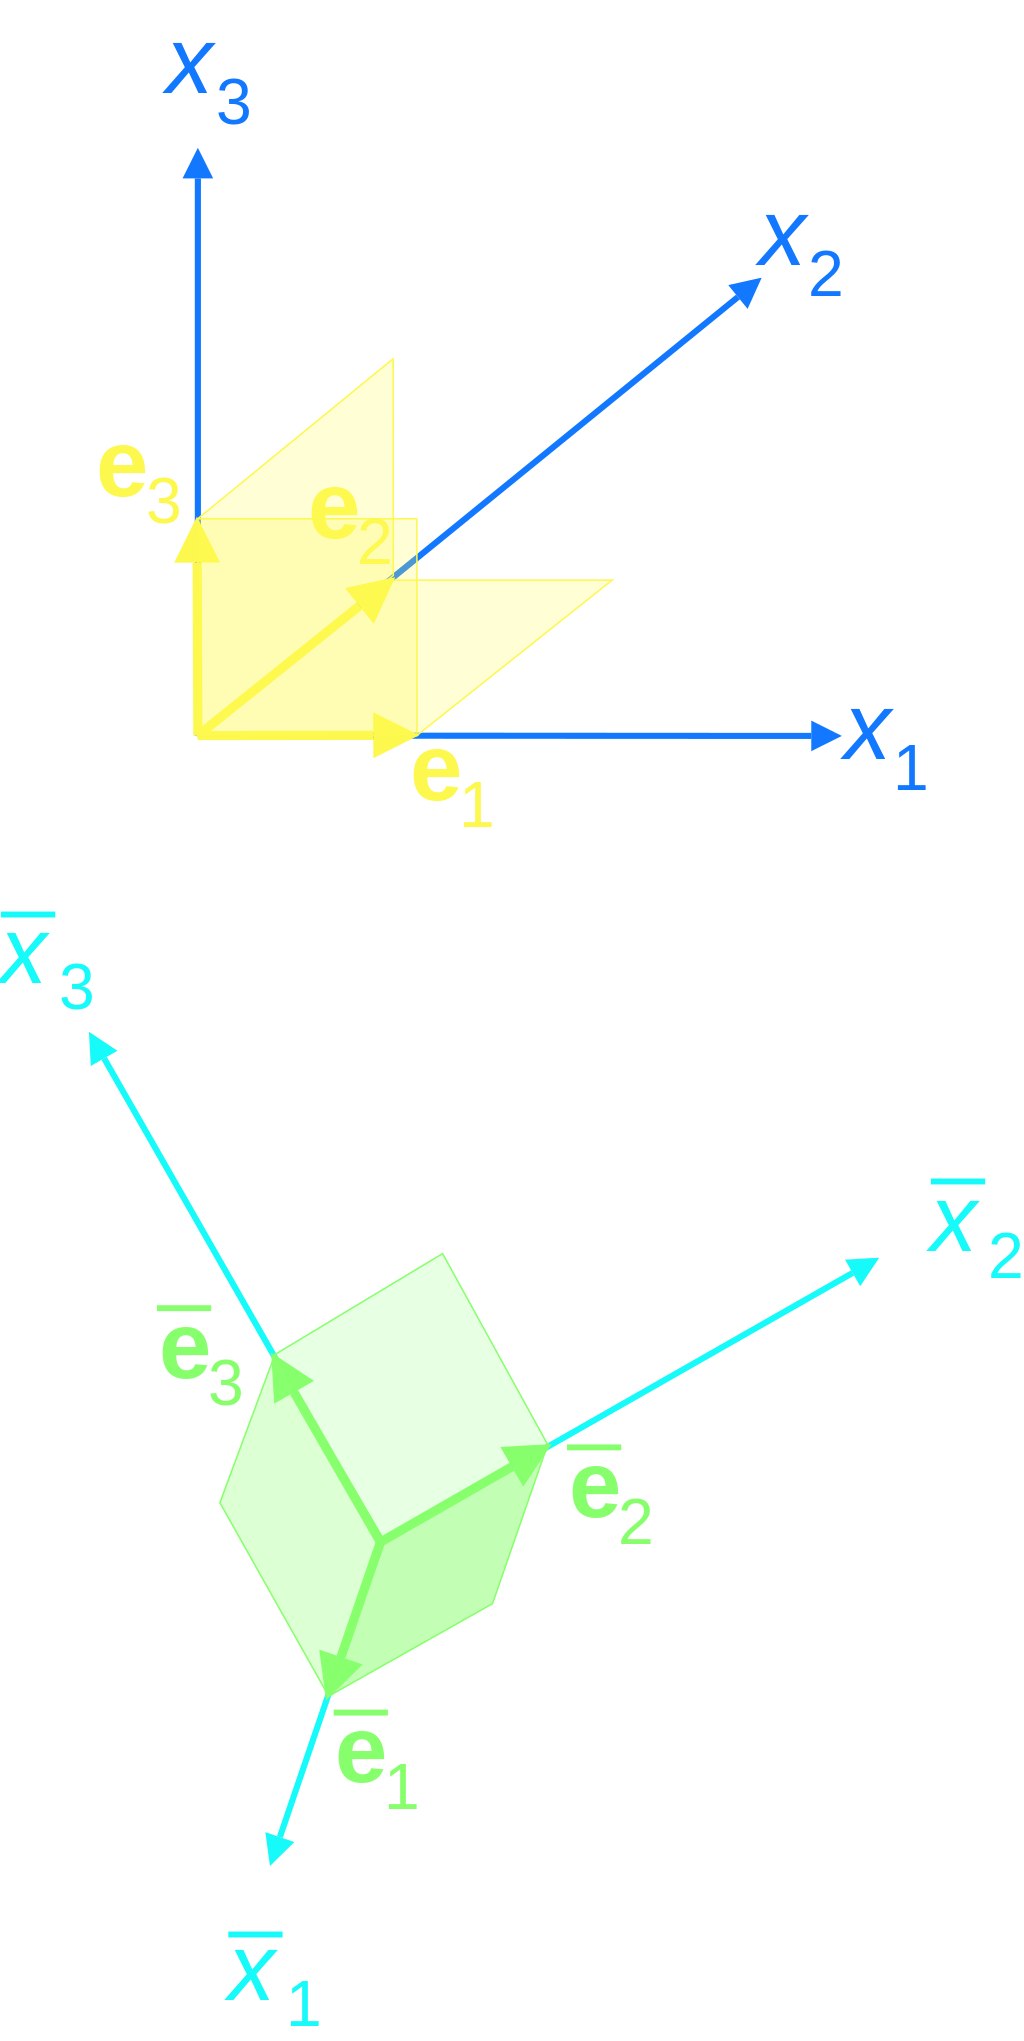
\includegraphics[scale=0.1]{./figures/Rectangular_coordinate_systems_index_lowered.png}
\end{center}
\end{frame}
%-------------- end slide -------------------------------%}}}
\section[\textcolor{yellow}{}]{\textcolor{yellow}{Fourier Expansion}}
%-------------- start slide -------------------------------%{{{ 20
\frame{
\frametitle{Fourier Expansion}
\pause
\begin{theorem}[Fourier Expansion]
  Let
  $\{ \vec{f}_1, \vec{f}_2, \ldots, \vec{f}_m \}$
  be an orthogonal basis of a subspace $U$ of $\RR^n$.
  Then for any $\vec{x}\in U$,
  \[ \vec{x} =
    \left(\frac{\vec{x}\dotprod\vec{f}_1}{|| \vec{f}_1 ||^2}\right) \vec{f}_1 +
    \left(\frac{\vec{x}\dotprod\vec{f}_2}{|| \vec{f}_2 ||^2}\right) \vec{f}_2 + \cdots +
    \left(\frac{\vec{x}\dotprod\vec{f}_m}{|| \vec{f}_m ||^2}\right) \vec{f}_m.
  \]
  This expression is called the \alert{Fourier expansion}
  of $\vec{x}$, and
  \[
    \frac{\vec{x}\dotprod\vec{f}_j}{|| \vec{f}_j ||^2},\quad j=1,2,\ldots,m
  \]
  are called the \alert{Fourier coefficients.}
\end{theorem}
}
%-------------- end slide -------------------------------%}}}
%-------------- start slide -------------------------------%{{{ 21
\frame{
\begin{example}
  Let $\vec{f}_1   = \left[\begin{array}{r} 1 \\ -1 \\ 2 \end{array}\right],
    \vec{f}_2      = \left[\begin{array}{r} 0 \\ 2 \\ 1  \end{array}\right]$,
  and $\vec{f}_3   = \left[\begin{array}{r} 5 \\ 1 \\ -2 \end{array}\right]$,
  and let $\vec{x} = \left[\begin{array}{r} 1 \\ 1 \\ 1 \end{array}\right]$.

  We have seen that $B=\{ \vec{f}_1, \vec{f}_2, \vec{f}_3\}$
  is an orthogonal subset of $\RR^3$.
  \medskip

  \pause
  It follows that $B$ is an orthogonal basis of $\RR^3$.
  (Why?)
  \pause
  \medskip

  To express $\vec{x}$ as a linear combination of the vectors of
  $B$, apply the {\it Fourier Expansion Theorem.}
  Assume $\vec{x}=t_1\vec{f}_1 + t_2\vec{f}_2 +t_3\vec{f}_3$.
  \pause
  Then
  \[
  t_1 =\frac{\vec{x}\dotprod\vec{f}_1}{||\vec{f}_1||^2} = \frac{2}{6},
  ~~t_2 =\frac{\vec{x}\dotprod\vec{f}_2}{||\vec{f}_2||^2} = \frac{3}{5},
  \quad\text{and}\quad
  t_3 =\frac{\vec{x}\dotprod\vec{f}_3}{||\vec{f}_3||^2} = \frac{4}{30}.\]
  \pause
  Therefore,
  \[ \left[\begin{array}{r} 1 \\ 1 \\ 1 \end{array}\right]
  = \frac{1}{3}\left[\begin{array}{r} 1 \\ -1 \\ 2 \end{array}\right]
  +\frac{3}{5}\left[\begin{array}{r} 0 \\ 2 \\ 1  \end{array}\right]
  +\frac{2}{15}\left[\begin{array}{r} 5 \\ 1 \\ -2 \end{array}\right].\]
\end{example}
}
%-------------- end slide -------------------------------%}}}
%-------------- start slide -------------------------------%{{{ 22
\frame{
\begin{proofnoend}[Fourier Expansion]
  Let $\vec{x}\in U$.
  Since $\{ \vec{f}_1, \vec{f}_2, \ldots, \vec{f}_m \}$ is a basis of
  $U$, $\vec{x}=t_1 \vec{f}_1 + t_2\vec{f}_2 + \cdots + t_m\vec{f}_m$
  for some $t_1, t_2, \ldots, t_m\in\RR$.
  \pause
  Notice that for any $i$, $1\leq i\leq m$,
  \begin{eqnarray*}
  \vec{x}\dotprod\vec{f}_i
  & = &
  (t_1 \vec{f}_1 + t_2\vec{f}_2 + \cdots + t_m\vec{f}_m)\dotprod\vec{f}_i\\
  \pause
  & = & t_i \vec{f}_i\dotprod\vec{f}_i ~~\mbox{ since }
  \{ \vec{f}_1, \vec{f}_2, \ldots, \vec{f}_m \}\mbox{ is orthogonal}\\
  & = & t_i ||\vec{f}_i||^2.
  \end{eqnarray*}
  \pause
  Since $\vec{f}_i$ is nonzero, we obtain
  \[ t_i = \frac{\vec{x}\dotprod\vec{f}_i}{||\vec{f}_i||^2}.\]
  The result now follows.
  \myQED
\end{proofnoend}
\pause
\vfill
\begin{remark}
If $\{ \vec{f}_1, \vec{f}_2, \ldots, \vec{f}_m \}$ is an orthonormal
basis, then the Fourier coefficients are simply
$t_j=\vec{x}\dotprod\vec{f}_j$, $j=1,2,\ldots,m$.
\end{remark}
}
%-------------- end slide -------------------------------%}}}
%-------------- start slide -------------------------------%{{{ 23
\frame{
\begin{problem}
      \vspace{-2em}
  \[
      \text{Let}\quad
      \vec{f}_1=\left[\begin{array}{r} 1 \\ 1 \\ 0 \\ 0 \end{array}\right],\quad
      \vec{f}_2=\left[\begin{array}{r} 1 \\ -1 \\ 0 \\ 0  \end{array}\right],\quad
      \vec{f}_3=\left[\begin{array}{r} 0 \\ 0 \\ 1 \\ 1  \end{array}\right],\quad
      \vec{f}_4=\left[\begin{array}{r} 0 \\ 0 \\ 1 \\ -1 \end{array}\right].
  \]
  Show that $B=\{ \vec{f}_1, \vec{f}_2, \vec{f}_3, \vec{f}_4\}$ is an
  orthogonal basis of $\RR^4$, and express
  $\vec{x}=\left[\begin{array}{cccc}
  a & b & c & d \end{array}\right]^T$ as a linear combination of
  $\vec{f}_1, \vec{f}_2, \vec{f}_3$ and $\vec{f}_4$.
\end{problem}
\pause
\vfill
\begin{solution}
  Computing $\vec{f}_i\dotprod\vec{f}_j$ for $1\leq i<j\leq 4$ gives us
  \[
      \begin{array}{rcrcrcrcrcr}
        \vec{f}_1\dotprod\vec{f}_2 & = & 0, \hspace*{.25in}
        \vec{f}_1\dotprod\vec{f}_3 & = & 0, \hspace*{.25in}
        \vec{f}_1\dotprod\vec{f}_4 & = & 0, \\[0.2em]
        \vec{f}_2\dotprod\vec{f}_3 & = & 0, \hspace*{.25in}
        \vec{f}_2\dotprod\vec{f}_4 & = & 0, \hspace*{.25in}
        \vec{f}_3\dotprod\vec{f}_4 & = & 0.
      \end{array}
  \]
  Hence, $B$ is an orthogonal set.
  \pause
  It follows that $B$ is independent, and since $|B|=4=\dim(\RR^4)$,
  $B$ also spans $\RR^4$.
  Therefore, $B$ is an orthogonal basis of $\RR^4$.
  \pause
  By the Fourier Expansion Theorem,
  \[
      \vec{x} = \left(\frac{a+b}{2}\right)\vec{f}_1
      +\left(\frac{a-b}{2}\right)\vec{f}_2
      +\left(\frac{c+d}{2}\right)\vec{f}_3
      +\left(\frac{c-d}{2}\right)\vec{f}_4.
  \]
  \myQED
\end{solution}
}
%-------------- end slide -------------------------------%}}}
\end{document}
